\subsection{System Characterisation}

After  a system's  step  response  has  been  measured,  it  is  necessary  to
characterise  and  determine  its  properties before it's possible  to  fit  a
transfer function to it. The method  of  characterisation used here is to find
the point of inflection in the measured step response, through which a tangent
is placed.  The  tangent's  intersection  points  with  the  lower  and  upper
horizontal bounds  are used to determine the dead time $T_u$ and the rise time
$T_g$.  Further, the amplitude $K_s$ of the step response can  be  determined.
This process is illustrated in figure \ref{fig:tu-tg-example}.

\begin{figure}[t]
    \centering
    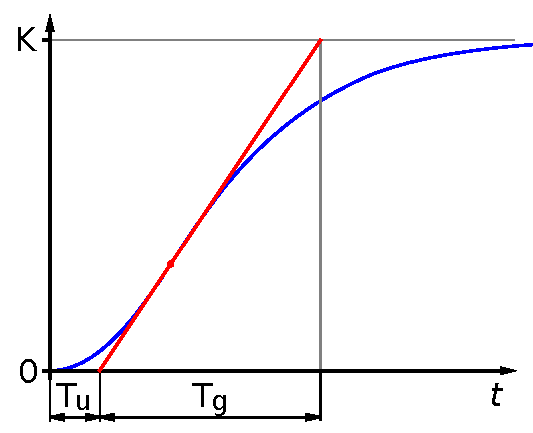
\includegraphics[width=\imagewidth]{images/tu_tg_example}
    \caption{Example step response of a system and measurement of the angle of inflection for determining $K_s$, $T_u$ and $T_g$. Image taken from Wikipedia\cite{ref:tu-tg}.}
    \label{fig:tu-tg-example}
\end{figure}

It is important to note that this method  of  characterisation  is  valid  for
systems  with  an  order of at least  2  that  don't  exhibit  any  overshoot.

\begin{figure}[t]
    \centering
    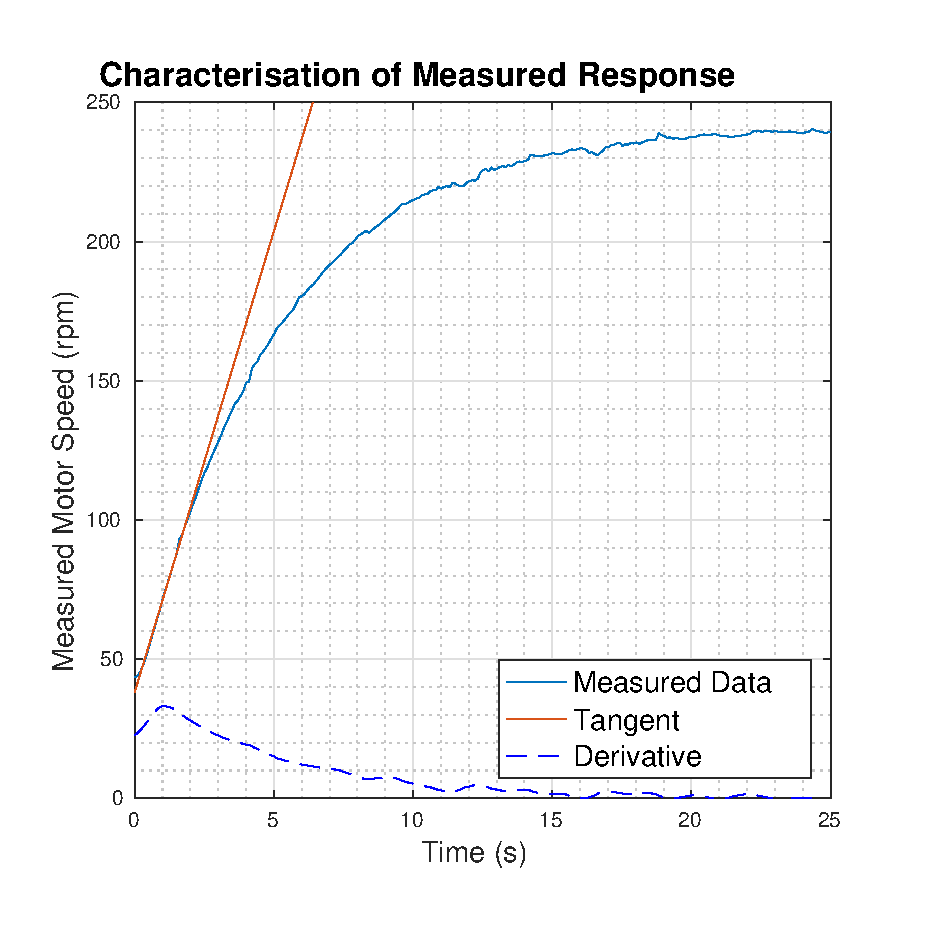
\includegraphics[width=\imagewidth]{images/characterisation}
    \caption{Calculated tangent of measured step response data.}
    \label{fig:characterisation}
\end{figure}

Using  MATLAB, the measured step response from the lab experiment is smoothed,
the derivative is computed to find the point of inflection, and the tangent is
calculated.   The    results    of    this    are    visualised    in   figure
\ref{fig:characterisation}.

Regarding the parameter $K_s$, a common pitfall is to  say  that  $K_s$ is the
total  change in the step response. This  statement  is  in  fact  false,  but
happens to yield the correct value as long as the input step  function  has an
amplitude of $1$, which unfortunately is the only case studied in the majority
of theory lectures. The parameter $K_s$ is in fact the total change in  output
divided by the total change in input:

\begin{equation}
    K_s = \frac{\Delta K_{out}}{\Delta K_{in}}
\end{equation}

The calculated values of $T_u$, $T_g$ and $K_s$ turn out to be:

\begin{align*}
    T_u &= 0.1655 \\
    T_g &= 5.9602 \\
    K_s &= 197.42
\end{align*}

